% Project report for clock-assisted consensus in OmniPaxos-KV
\documentclass{article}
\usepackage[utf8]{inputenc}
\usepackage{graphicx}

\title{Clock-Assisted Consensus in OmniPaxos-KV with Nezha-style Deadline-Ordered Multicast}
\author{Lorenzo Deflorian, Riccardo Fragale, Jouzas Skarbalius}
\date{\today}

\begin{document}

\maketitle

\section{Introduction}
Large-scale distributed systems increasingly rely on consensus protocols to provide strongly consistent services over unreliable networks. Classical leader-based protocols such as Paxos and Raft guarantee linearizability but often pay a performance cost: every client operation typically requires at least two round trips to the leader, and network reordering or failures can further increase latency. Recent work on clock-assisted consensus, in particular the Nezha protocol, demonstrates that when nodes share tightly synchronized clocks, it becomes possible to speculatively process requests in deadline order and obtain a fast path that completes in effectively one round trip.

This project explores the hypothesis that \emph{better clock synchronization leads to better consensus performance}. Building on the OmniPaxos-KV codebase, we integrate a configurable clock simulator and a Nezha-inspired, deadline-ordered multicast (DOM) layer into the existing key-value store. Our design uses synchronized logical clocks to attach deadlines to client requests and enforces a global ordering based on those deadlines, while preserving linearizability even when clock quality is poor or the network behaves adversarially.

Concretely, we extend OmniPaxos-KV with three main components. First, we implement a pluggable clock simulator that models drift, synchronization frequency, and uncertainty bounds, and exposes a simple API to the rest of the system. Second, we introduce a DOM-like layer that buffers and releases requests in deadline order, providing an optimistic fast path when requests arrive on time. Third, we modify the proxy and server logic to support a fast path---where a quorum of replicas speculatively execute and reply early---and a slow path, where the system safely falls back to normal OmniPaxos log replication whenever deadlines are missed or ambiguity arises.

We evaluate our design using a suite of benchmarks that vary clock quality, deadline strategy, and failure conditions. All experiments are run with a fixed deployment of three servers, two clients, and one proxy. Our results show that tighter clock synchronization and adaptive deadline selection increase the fraction of operations that complete on the fast path, thereby improving both latency and throughput, while the system remains linearizable under clock skew and node failures by transparently switching to the slow path when necessary.

\section{Design}
Our design adds a Nezha-style, clock-assisted fast path on top of the existing OmniPaxos-KV architecture. The key idea is to use synchronized clocks to tag each client request with a deadline and to ensure that servers process requests in increasing deadline order whenever they arrive on time. When this optimistic assumption fails, the system reverts to a conservative slow path that is backed by standard OmniPaxos log replication.

\subsection{Clock Simulator}
The foundation of our design is a configurable clock simulator, exposed through the \texttt{ClockSim} interface. Each node maintains its own simulated clock, parameterized by a drift rate, an uncertainty bound, and a synchronization frequency. The drift rate controls how quickly the simulated time deviates from real time, while the synchronization frequency determines how often the clock is ``pulled'' back towards a reference time. The uncertainty bound represents the maximum deviation that upper layers must assume when reasoning about deadlines.

The simulator provides two main methods, \texttt{get\_time()} and \texttt{get\_uncertainty()}, which return the current simulated time (in microseconds) and the current uncertainty estimate, respectively. All components that need time, notably the proxy and the DOM layer on the servers, depend exclusively on this interface rather than on the system clock. This lets us experiment with different clock qualities and resynchronization intervals without changing the rest of the code.

\subsection{DOM-style Deadline-Ordered Processing}
On top of the clock simulator, we implement a Nezha-inspired, DOM-like message processing layer. The proxy assigns each incoming client request a send time and a deadline, and forwards the request as a DOM message to all servers. Each server maintains two logical buffers:

\begin{itemize}
  \item \textbf{Early buffer}: a priority queue ordered by deadline (and implicitly by client and request identifiers). Requests that arrive before their deadlines are inserted into this buffer. The DOM layer periodically checks the earliest pending deadline and releases all requests whose deadlines have been reached, preserving increasing deadline order.
  \item \textbf{Late buffer}: a secondary store for requests that cannot be safely inserted into the early buffer, for example because they arrive after their deadline or because they would violate the monotonicity of deadlines. These requests are not processed on the fast path but may still be committed later via the slow path.
\end{itemize}

The server event loop queries the DOM layer for the duration until the next deadline and sleeps accordingly. When a deadline expires, the DOM layer returns a batch of \emph{committable} messages from the early buffer. This provides a deterministic, deadline-based order that is consistent across replicas as long as messages arrive on time and within the uncertainty window.

\subsection{Proxy-Centered Fast and Slow Paths}
The proxy is responsible for interfacing with clients and orchestrating fast and slow paths. When a client sends a write or read request, the proxy records the current simulated time and computes a deadline using either a fixed default value or an adaptive value learned from previous runs (Section~\ref{subsec:adaptive-deadlines}). From this, it also derives a fast-path timeout that bounds how long it is willing to wait for fast replies from the servers.

The proxy then multicasts the DOM-annotated request to all servers. As fast replies arrive, the proxy groups them per client request and tracks how many matching responses have been received. If a super-quorum of consistent fast replies is gathered before the fast-path timeout, the proxy concludes that the request has been safely processed in deadline order and replies to the client with the result. If the timeout expires or conflicting information is observed, the proxy aborts the fast path for that request and emits a slow-path abort message to all servers. This triggers a fallback where the request is ordered and committed through the OmniPaxos log and the client receives a slow-path reply once the decision is durable.

\subsection{Adaptive Deadlines and One-Way Delay Estimation}
\label{subsec:adaptive-deadlines}
Static deadlines must trade off between two conflicting goals: they must be long enough to tolerate network jitter and clock uncertainty but short enough to avoid adding unnecessary waiting time. To better navigate this trade-off, our design includes an adaptive deadline mechanism based on one-way delay (OWD) estimation.

Servers locally measure apparent OWDs between the proxy and each server by comparing send and receive timestamps. These samples are fed into a per-node sliding window maintained by an \texttt{Owd} component. For each node, the \texttt{Owd} structure maintains a bounded window of recent delay samples and computes a percentile (e.g., the median or 95th percentile) over that window. The proxy collects these measurements, maintains per-node deadline estimates, and tracks the maximum observed value across servers.

When computing a deadline for a new request, the proxy either uses a static default value or, if sufficient OWD samples are available and adaptive mode is enabled, uses the learned maximum percentile-based estimate. This follows the spirit of Nezha's percentile-based deadline calculation but in a simplified form that is easy to integrate with OmniPaxos-KV. In practice, this adaptive strategy increases the fast-path ratio in stable conditions while still reacting to changes in network conditions and clock quality.

\subsection{End-to-End Fast and Slow Path Flows}
End-to-end, the system behaves as follows. On the \emph{fast path}, a client submits a request to the proxy, which timestamps and deadlines it, then multicasts it as a DOM message to all servers. Each server inserts the message into its early buffer, and once the deadline is reached, the DOM layer releases it in deadline order. The leader speculatively executes the request against its local key-value state and responds to the proxy, while followers verify the ordering and send fast replies. The proxy aggregates these replies and, if a sufficient number of consistent responses arrive before the fast-path timeout, returns a fast-path response to the client.

On the \emph{slow path}, if the proxy detects that the fast-path timeout has been exceeded or that the deadline could not be respected, it aborts the fast path for that request and broadcasts an abort message to all servers. The servers then ensure that the request is properly ordered and durably decided through the OmniPaxos log. Once the decision is committed, the server generates a slow-path reply containing the final result and sends it back to the proxy. This guarantees linearizability even in the presence of poor clock synchronization, network reordering, or node failures, at the cost of higher latency.

\section{Implementation}
In this section we describe how the above design is realized within the OmniPaxos-KV codebase and how the main components interact. Our implementation reuses the existing networking and storage infrastructure as much as possible, and introduces new modules for clock simulation, deadline-based ordering, and adaptive deadline computation.

\subsection{Clock Simulator and Configuration}
The clock simulator is implemented as a reusable \texttt{ClockSim} type, parameterized by three values: drift rate, uncertainty bound, and synchronization frequency. These parameters are loaded from configuration files and from a dedicated \texttt{ClockConfig} structure. The simulator maintains internal state to track when the last synchronization occurred and how much drift has accumulated since then. Whenever \texttt{get\_time()} is called, the simulator updates its internal time based on the configured drift rate and potentially triggers a resynchronization if the synchronization interval has elapsed.

To validate the simulator, we provide unit tests that check monotonicity, ensure that synchronization reduces large drift errors, and verify that configuration files are parsed correctly. Additional tests instantiate multiple clocks with different drift parameters and confirm that, after synchronization, their simulated times converge within a small tolerance.

\subsection{One-Way Delay Estimation}
Adaptive deadline computation relies on measuring and aggregating OWD samples. We implement this in a separate \texttt{Owd} module that manages, for each node, a bounded deque of recent delay values. When a new sample is added, the module either pushes it to the back of the deque (if the window is not full) or drops the oldest sample to maintain the window size. To compute an adaptive deadline estimate for a node, the module copies the stored values into a temporary vector, selects the configured percentile using an efficient selection operation, and returns the resulting value. If no samples are available, the module falls back to a configured default deadline.

On the server side, OWD samples are recorded whenever a fast reply is generated. The proxy receives these replies, extracts the per-node deadline lengths, and updates its record of the maximum observed deadline across servers. This maximum value is then used as the adaptive deadline for subsequent client requests.

\subsection{Proxy Logic}
The proxy component is implemented as an asynchronous task that listens for client messages and server replies over existing network channels. When a client issues an append operation, the proxy constructs a unique key from the client identifier and command identifier, records the request in its internal state, and queries the clock simulator for the current time. It then chooses a deadline, either the configured default or the current maximum adaptive estimate, and computes a fast-path timeout as a function of the deadline and the expected round-trip time.

The proxy wraps the client message into a DOM message that includes the client identifier, command identifier, payload, send time, and deadline, and multicasts this message to all servers. For each in-flight request, the proxy maintains a reply set that groups fast replies by their content and tracks when enough consistent responses have been observed. A periodic timer checks for fast-path timeouts and triggers fast-path aborts when necessary. In that case, the proxy removes the fast-path reply set, marks the request as aborted, and sends an abort message back to all servers, signalling that the slow path should be used.

\subsection{Server Event Loop and DOM Integration}
On the server side, we extend the existing OmniPaxos server to integrate the DOM layer and the proxy interactions. Each server runs an event loop that multiplexes several concerns: receiving cluster messages for OmniPaxos, receiving client messages, receiving proxy messages, performing leader election, draining the late buffer, and handling DOM deadlines. The server constructs a \texttt{Dom} instance configured with the same clock and OWD parameters as the proxy.

When a DOM message arrives from the proxy, the server inserts it into the appropriate buffer. Periodically, the server queries the DOM layer for the duration until the next deadline and sleeps until that instant. When the sleep elapses, the server calls \texttt{handle\_deadline()}, which returns the set of messages whose deadlines have just passed. For each such message, the server constructs a command for OmniPaxos and, depending on whether it is currently the leader, either speculatively executes the command and sends a fast reply or simply sends a fast reply and defers durable commitment. OmniPaxos eventually decides the same command sequence, allowing followers and lagging nodes to catch up.

The server also handles slow-path aborts from the proxy. Upon receiving an abort message for a given request, the server removes any optimistic state associated with that request and ensures that the command is appended to the OmniPaxos log in the correct position. Once the decision is committed, the server generates a slow-path reply containing the final result and sends it back to the proxy.

\subsection{Client Behaviour}
Clients are implemented as lightweight asynchronous processes that send a mix of read and write requests according to a configurable workload pattern. Each client connects either directly to the servers or, in our experiments, via the proxy. Before starting the workload, clients wait for a start signal broadcast by the servers, ensuring that all nodes begin the experiment in a synchronized fashion.

During the experiment, clients generate requests at configured intervals and with a controlled read/write ratio. Each request is tagged with a monotonically increasing identifier and a key derived from that identifier. For writes, the client stores the value it expects to be written so that responses can be validated. As responses arrive---either directly from servers or via the proxy---the client records their latency and correctness in a \texttt{ClientData} structure and eventually persists this information to disk for offline analysis.

\section{Testing}
Testing focuses on two complementary aspects: validating that the clock simulator and DOM layer behave as intended, and verifying that the overall system remains linearizable under a variety of timing and failure scenarios.

\subsection{Clock Simulator Tests}
We first validate the clock simulator in isolation using unit tests. These tests instantiate \texttt{ClockSim} with different drift rates, uncertainty bounds, and synchronization frequencies, and check several properties:

\begin{itemize}
  \item \textbf{Monotonicity}: consecutive calls to \texttt{get\_time()} must never go backwards, even when the simulator performs a resynchronization.
  \item \textbf{Drift correction}: for large drift rates combined with periodic synchronization, the effective time difference over a given real-time interval should remain bounded, demonstrating that synchronization corrects accumulated drift.
  \item \textbf{Configuration parsing}: \texttt{ClockConfig} instances loaded from configuration files must match expected values, and invalid configurations (e.g., zero synchronization frequency) must be rejected.
  \item \textbf{Convergence}: separate \texttt{ClockSim} instances with very different drift rates but the same synchronization frequency are shown to converge to similar times after a synchronization event.
\end{itemize}

These tests give confidence that the simulated clocks match our intended error model and that their parameters are correctly wired to configuration files.

\subsection{DOM and Proxy--Server Integration Tests}
To validate the DOM layer and its integration with the proxy and servers, we rely on a combination of targeted tests and end-to-end experiments. At the DOM level, we verify that messages inserted into the early buffer are released in non-decreasing deadline order and that late arrivals are redirected to the late buffer. We also test that the duration until the next deadline is correctly computed, so that the server event loop wakes up exactly when necessary to process pending requests.

At the proxy and server level, we check that fast-path aborts are triggered correctly when deadlines or fast-path timeouts are exceeded, that abort messages are propagated to all servers, and that slow-path replies are eventually generated once OmniPaxos has committed the corresponding log entries. Logging and metrics are used extensively during development to confirm that requests that are executed on the fast path are not re-applied on the slow path and that the key-value state remains consistent.

\subsection{Benchmark Scenarios}
For a more realistic evaluation, we run a suite of benchmarks that exercise different clock qualities and fault conditions. Each benchmark is defined by a set of configuration files specifying the clock parameters, server and client behaviour, and proxy settings. All experiments use three servers, two clients, and one proxy. We focus on the following configurations:

\begin{itemize}
  \item \textbf{High quality}: small uncertainty and frequent resynchronization, modelling tightly synchronized clocks with low drift.
  \item \textbf{Medium quality}: moderate uncertainty and synchronization intervals, representing more typical data center conditions.
  \item \textbf{Low quality}: large uncertainty and infrequent synchronization, simulating poor clock synchronization.
  \item \textbf{Adaptive deadline}: the proxy uses OWD-based adaptive deadlines instead of a fixed default, aiming to improve the fast-path ratio while keeping waiting times reasonable.
  \item \textbf{Clock skew test}: deliberately introduces clock skew between nodes to stress the DOM layer's assumptions about shared time.
  \item \textbf{Node failure test}: injects server failures with configured probabilities and downtime durations to test robustness under crashes.
\end{itemize}

For each scenario, we configure the clients to generate a mix of read and write requests over a fixed duration, and we record client-side latencies, per-request outcomes, and server-side metrics such as fast-path and slow-path rates.

\subsection{Correctness and Linearizability}
To verify correctness, we collect detailed histories of client operations, including invocation and response times as well as the values returned by reads. These histories are fed into a linearizability checker inspired by the Nezha evaluation harness, which systematically explores whether there exists a serialization consistent with real-time ordering that explains the observed behaviour.

Across all benchmark scenarios considered in this report, the histories are found to be linearizable. In particular, even in the presence of significant clock skew and injected node failures, the system preserves linearizability by falling back to the slow path whenever speculative assumptions about deadlines are violated. This confirms the intended property that clocks are used purely to optimize performance, while safety is always guaranteed by the underlying OmniPaxos log replication.

\section{Testing Results}
In this section we summarize the performance of our clock-assisted consensus implementation under different clock qualities and fault conditions. For each configuration we report the total number of operations, the mix of puts and gets, end-to-end latency percentiles, fast-path usage, and throughput, and we interpret these results in light of our design.

\begin{table}[h]
  \centering
  \small
  \resizebox{0.95\textwidth}{!}{%
    \begin{tabular}{l r r r r r r r r l}
      \hline
      Config & Ops & Puts & Gets & p50 & p95 & p99 & Fast-path [\%] & Throughput [req/s] & Lin. \\
      \hline
      adaptive\_deadline & 364 & 274 & 90 & 4.46 & 9.71 & 15.52 & 77.7 & 17.1 & PASS \\
      high\_quality      & 362 & 180 & 182 & 4.26 & 7.60 & 10.07 & 83.4 & 17.9 & PASS \\
      low\_quality       & 363 & 271 & 92 & 5.96 & 13.63 & 15.31 & 69.7 & 17.3 & PASS \\
      medium\_quality    & 362 & 274 & 88 & 3.88 & 8.14 & 14.24 & 79.6 & 18.9 & PASS \\
      clock\_skew        & 362 & 264 & 98 & 4.60 & 6.46 & 13.88 & 51.4 & 19.5 & PASS \\
      node\_failure      & 402 & 304 & 98 & 9.78 & 2014.19 & 2814.55 & 2.0 & 16.8 & PASS \\
      \hline
    \end{tabular}
  }
  \caption{Summary of benchmark results across all configurations. Latencies are in milliseconds.}
\end{table}

\subsection{Adaptive Deadline}
Under the \emph{adaptive deadline} configuration, the system processes 364 operations, with 274 puts and 90 gets. The median end-to-end latency is approximately 4.46\,ms, with 95th and 99th percentiles of 9.71\,ms and 15.52\,ms, respectively. About 78\% of operations complete on the fast path, and the overall throughput is around 17\,requests per second. These results indicate that percentile-based OWD estimation allows the proxy to choose deadlines that are long enough to accommodate typical network and clock variability, thereby enabling a high fast-path ratio, while still keeping median latency in the low milliseconds.

\subsection{High-Quality Clocks}
In the \emph{high-quality} configuration, clocks exhibit low drift and tight uncertainty bounds with frequent resynchronization. Here the system executes 362 operations, roughly evenly split between 180 puts and 182 gets. Latencies improve compared to the adaptive configuration: the median is 4.26\,ms, with 95th and 99th percentiles at 7.60\,ms and 10.07\,ms. The fast-path ratio increases to about 83\% of operations, and throughput rises to approximately 18\,requests per second. This behaviour matches the project hypothesis: better clock synchronization and lower uncertainty allow more requests to be safely processed using the fast path, reducing both average and tail latencies.

\subsection{Low-Quality Clocks}
The \emph{low-quality} configuration uses clocks with larger uncertainty and less frequent synchronization. Under these conditions, the system handles 363 operations (271 puts and 92 gets). The median latency degrades to 5.96\,ms, with 95th and 99th percentiles at 13.63\,ms and 15.31\,ms, respectively. The fast-path ratio drops to about 70\%, and throughput is roughly 17\,requests per second. Compared to the high-quality case, we observe a clear shift: more operations fall back to the slow path because deadlines must be longer and are more frequently violated, which directly increases both median and tail latencies.

\subsection{Medium-Quality Clocks}
With \emph{medium-quality} clocks, which sit between the previous two extremes, the system processes 362 operations (274 puts and 88 gets). Latency results lie between the high- and low-quality cases: the median is 3.88\,ms, and the 95th and 99th percentiles are 8.14\,ms and 14.24\,ms. The fast-path ratio is approximately 80\%, and throughput reaches around 19\,requests per second. This intermediate configuration provides the best throughput among the fixed-deadline runs, illustrating that there is a sweet spot where deadlines are tight enough to avoid unnecessary waiting but still robust against typical jitter, maximizing fast-path usage.

\subsection{Clock Skew}
The \emph{clock skew} test deliberately introduces skew between node clocks while keeping other parameters comparable. In this scenario, the system again processes 362 operations, with 264 puts and 98 gets. The median latency is 4.60\,ms, while the 95th and 99th percentiles are 6.46\,ms and 13.88\,ms. The fast-path ratio decreases to about 51\%, and throughput is around 19\,requests per second. Despite the reduced fast-path usage, throughput remains competitive because many operations still meet their deadlines; however, the increased skew causes more requests to be redirected to the slow path, illustrating how the system gracefully degrades performance while preserving correctness when shared-time assumptions are violated.

\subsection{Node Failures}
Finally, the \emph{node failure} configuration injects server failures with a certain probability and downtime, stressing both the DOM layer and the underlying OmniPaxos consensus. Here the system executes 402 operations, with 304 puts and 98 gets. Latencies are significantly affected: the median is 9.78\,ms, while the 95th and 99th percentiles increase dramatically to 2{,}014.19\,ms and 2{,}814.55\,ms, respectively. Only about 2\% of operations complete on the fast path, and throughput is approximately 17\,requests per second. Most operations therefore fall back to the slow path and must wait for leader re-election and log commitment, leading to very high tail latencies. Nevertheless, all operations remain linearizable, demonstrating that the system maintains its safety guarantees even under severe failure conditions.

\subsection{Global Comparison}
Taken together, these results support the central hypothesis that clock quality and deadline selection have a strong impact on consensus performance. Configurations with better-synchronized clocks or well-chosen adaptive deadlines achieve higher fast-path ratios, lower median latencies, and improved throughput. As clock quality degrades, or as skew and failures are introduced, the system falls back more frequently to the slow path, causing performance to decline---especially at the tail---but without compromising linearizability. All configurations evaluated in this report passed linearizability checks, reinforcing the design principle that clocks are used solely to optimize performance while correctness is always enforced by the underlying consensus protocol.

\begin{figure}[h]
  \centering
  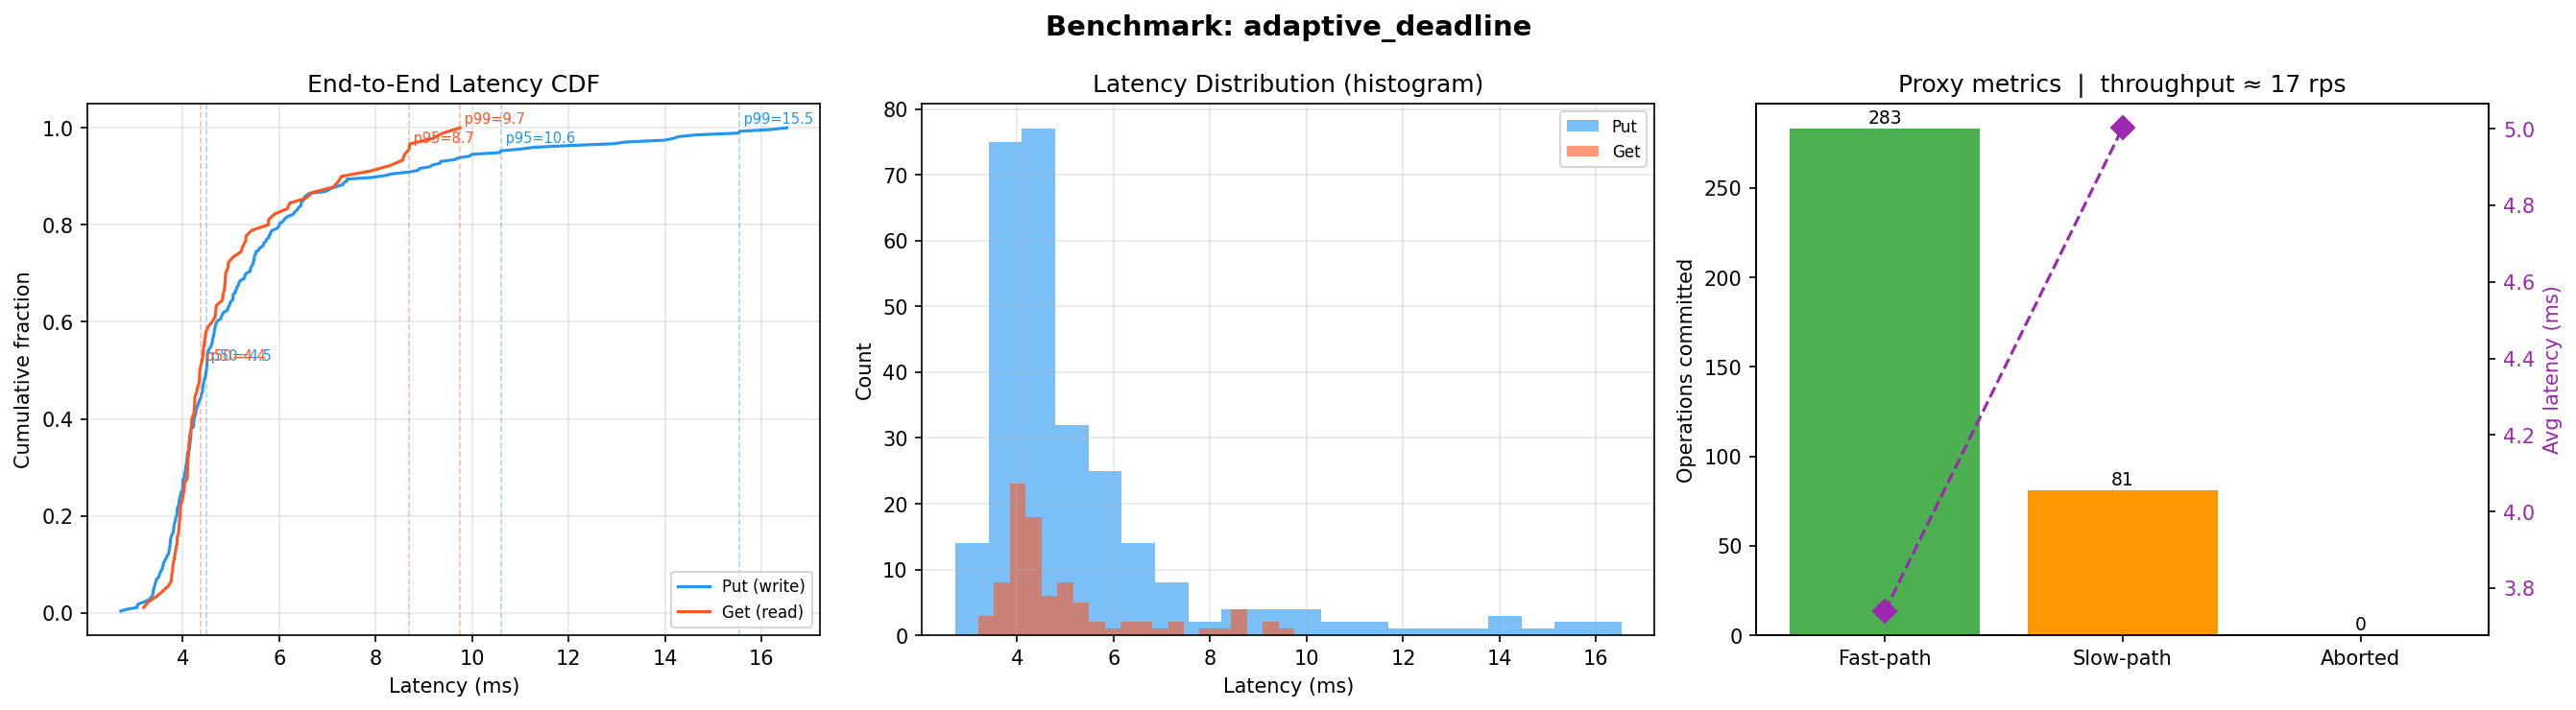
\includegraphics[width=0.8\textwidth]{data/adaptive_deadline/benchmark_results.png}
  \caption{Latency and throughput for the adaptive deadline configuration.}
\end{figure}

\begin{figure}[h]
  \centering
  
\includegraphics[width=0.8\textwidth]{data/high_quality/benchmark_results.png}
  \caption{Latency and throughput for the high-quality clock configuration.}
\end{figure}

\begin{figure}[h]
  \centering
  
\includegraphics[width=0.8\textwidth]{data/low_quality/benchmark_results.png}
  \caption{Latency and throughput for the low-quality clock configuration.}
\end{figure}

\begin{figure}[h]
  \centering
  
\includegraphics[width=0.8\textwidth]{data/medium_quality/benchmark_results.png}
  \caption{Latency and throughput for the medium-quality clock configuration.}
\end{figure}

\begin{figure}[h]
  \centering
  
\includegraphics[width=0.8\textwidth]{data/test_clock_skew/benchmark_results.png}
  \caption{Latency and throughput for the clock skew test configuration.}
\end{figure}

\begin{figure}[h]
  \centering
  
\includegraphics[width=0.8\textwidth]{data/test_node_failure/benchmark_results.png}
  \caption{Latency and throughput for the node failure configuration.}
\end{figure}

\section{Future Work}
There are several directions in which this work could be extended. First, our adaptive deadline mechanism uses a relatively simple percentile-based OWD estimator per node. Future work could explore more sophisticated estimators that account for correlations between paths, time-of-day effects, or sudden network changes, and that consider different percentiles depending on workload or service-level objectives. It would also be interesting to validate these mechanisms against real-world clock-synchronization protocols rather than simulated clocks.

Second, the current implementation treats all operations uniformly, regardless of whether they commute. Techniques from Nezha that exploit operation commutativity could allow additional reordering flexibility, increasing the fast-path ratio without endangering correctness. Integrating such optimizations into OmniPaxos-KV would require extending the key-value interface with richer semantics and updating the DOM layer accordingly.

Third, our failure model is limited to crash failures and static cluster membership. Extending the system to handle dynamic reconfiguration, network partitions, and more realistic failure injection patterns would better approximate production environments. Coupling this with richer telemetry and online monitoring of fast- versus slow-path usage could enable automatic tuning of deadline parameters in response to changing conditions.

\section{Summary}
This project integrates Nezha-style, clock-assisted consensus ideas into the OmniPaxos-KV key-value store. We implement a configurable clock simulator, a DOM-like deadline-ordered processing layer, adaptive deadline computation based on one-way delays, and proxy and server logic that support both optimistic fast paths and conservative slow paths. Using a suite of benchmarks that vary clock quality, deadline strategy, and fault conditions, we show that better clock synchronization and well-tuned deadlines substantially increase the fraction of operations that complete on the fast path, thereby improving latency and throughput.

At the same time, the system remains linearizable even when clocks are poor, skewed, or when node failures occur, by safely falling back to the slow path and relying on OmniPaxos log replication for ordering and durability. These results confirm that clock information can be exploited to accelerate consensus without compromising correctness, and they highlight the importance of jointly designing clock synchronization, deadline selection, and consensus mechanisms in modern distributed systems.

\end{document}

